% Machines-targeted research manuscript work draft, 2026-10-20.
% Free-format FIRST submission is permitted by Machines author instructions.
% Before submission: migrate to official MDPI LaTeX template and confirm all metadata.
% Every item marked DATA REQUIRED must be resolved from real logged evidence.
\documentclass[11pt,a4paper]{article}
\usepackage[margin=2.35cm]{geometry}
\usepackage{amsmath,amssymb,bm,graphicx,booktabs,multirow,array,xcolor,hyperref}
\usepackage{enumitem}
\usepackage{caption}
\setlength{\parskip}{0.34em}
\setlength{\parindent}{0pt}
\hypersetup{colorlinks=true,urlcolor=blue,linkcolor=blue,citecolor=blue}
\newcommand{\SE}{\mathrm{SE}(3)}
\newcommand{\R}{\mathbb{R}}
\newcommand{\Img}{J_{\mathrm{img}}}
\newcommand{\todoexp}[1]{\textcolor{red!70!black}{\textbf{[DATA REQUIRED: #1]}}}
\title{Compensation-Aware Gait Adaptation for Camera-Stable Hexapod Locomotion on Uneven Terrain}
\author{Author names and affiliations pending author confirmation}
\date{Internal research draft --- 20 October 2026 --- not for submission}
\begin{document}
\maketitle
\begin{abstract}
Uneven-terrain locomotion introduces gait-synchronous camera motion that can affect visual sensing on hexapod robots with rigidly mounted cameras. Body-pose stabilization can attenuate some of this disturbance, but its achievable correction depends on support contacts, joint workspace, and actuator response. We investigate a gait selection principle that evaluates candidate gaits according to the \emph{predicted residual image-plane disturbance after feasible body compensation}, rather than the disturbance before compensation. The proposed framework evaluates gait candidates through a lightweight, gait-conditioned model of raw image disturbance and the achieved closed-loop response of a fixed body stabilizer. A supervisory controller selects gait frequency, stance duty factor, and a touchdown-profile parameter under locomotion progress, foot-clearance, contact and joint limits. Image-space residual motion is separated from the expected optical flow of the navigation task. The planned evaluation comprises paired multi-terrain dynamics simulations, strong fixed-gait and sequential-optimization baselines, and synchronized camera--IMU robot demonstrations. \textbf{This is a methods-first manuscript draft; quantitative outcome statements must be added only after actual experiments.}
\end{abstract}
\noindent\textbf{Keywords:} hexapod locomotion; adaptive gait; visual stability; body-pose compensation; image motion; constrained optimization.
\section{Introduction}
Walking over irregular ground can cause a rigidly mounted camera to undergo periodic translation and rotation during swing--stance transitions, body weight transfer, and foot touchdowns. For an onboard imaging system, the consequences include unwanted inter-frame motion and image motion during exposure. These effects are relevant even when the robot successfully tracks its commanded velocity and its mean roll or pitch remains near zero.

One response is to exploit the leg configuration to stabilize the body. However, stance feet constrain the available movement, and the remaining joint workspace changes throughout the gait. The motions required for gaze direction, obstacle clearance, and velocity tracking may compete for the same joints. Under these conditions, camera stabilization is not an independently actuated task as it would be with a dedicated gimbal.

Existing work has shown that legged robots can adjust body pose for directed vision \cite{shaw2019}, that gait learning can improve image-based perception \cite{saggar2007}, and that hexapod mechanical and gait parameters can be optimized to reduce body oscillations \cite{burkus2022,yin2024}. Hence neither visual objectives nor gait adaptation nor their generic combination can be presented as novel. The unresolved engineering decision addressed here is more specific: \emph{when two feasible gaits generate different disturbances and leave different body-correction authority, which gait yields the smaller camera disturbance after the body controller has acted?}

A gait producing the smallest uncontrolled angular-velocity norm need not minimize residual image motion. A larger, slow oscillation may be easy to compensate if the support configuration provides sufficient workspace, whereas a smaller but fast disturbance or a disturbance occurring at a constrained contact phase may remain in the camera image. Conversely, a candidate with favorable raw motion may consume nearly all the joint motion needed for stabilization. This creates a coupling between gait selection and the actual body-correction mechanism.

We propose a controller that predicts gait-conditioned camera disturbance, approximates how much of that disturbance a fixed, project-owned body-pose compensator can cancel under support and actuator constraints, and selects a feasible gait based on the predicted remaining image motion. This compensator is a planned research component, not an existing executable in the current standalone runner. The local image interaction model supplies a task-dependent projection of camera motion; it is not used to claim that a rigid camera requires high-rate image feedback. RGB image measurements are instead retained for correction, calibration, and independent validation.

The manuscript is organized around two technical propositions to be tested: (i) candidate-specific feasible compensation changes the ranking of gaits compared with ranking by uncompensated body motion; and (ii) using this ranking online improves image motion under matched achieved travel speed, without materially reducing terrain traversal success. The experiments and statistical comparisons needed for these propositions are specified in Section~\ref{sec:experiments}, and no empirical superiority is assumed in advance.

\section{Related Work}
\subsection{Legged gaze and camera stabilization}
Shaw et al. developed workspace CPG with SE(3) body-pose control on an 18-DOF hexapod, enabling online visually guided locomotion and directed gaze without an independent camera actuator \cite{shaw2019}. It is therefore incorrect to distinguish our study by claiming that earlier controllers used only inertial sensing or did not alter CPG motion using vision. The proposed distinction is the downstream residual pixel-motion criterion and its explicit dependence on the compensation limits of each gait candidate. Earlier camera-oriented gait learning also exists: Saggar et al. jointly optimized speed and visual stability on an Aibo quadruped and demonstrated a perception benefit \cite{saggar2007}. That study is a substantive precedent for image-quality-aware gait search.

Motion-blur-constrained visual control has also been formulated as an optimization problem; Robic et al. incorporated a blur-related constraint into QP visual servoing \cite{robic2024}. Thus the use of a camera-space cost or of a constrained optimization solver is an established technique. Our objective is not a new visual servo controller but a locomotion-specific choice among disturbances that can or cannot be compensated by the body.

\subsection{Hexapod gait and body coordination}
Burkus et al. explicitly minimized unwanted body motion, including the sensor consequences of vibration, while co-optimizing structural and walking parameters \cite{burkus2022}. Smart Gait addressed hexapod swing trajectories and gait tuning to reduce mechanical costs and improve locomotion behavior \cite{yin2024}. Gao et al. combined gait planning, smoothed foot trajectories and contact-related compliant control to improve motion stability \cite{gao2022}. These studies preclude claims that we are first to reduce vibration at its source by changing a walking gait.

Yu et al. coordinated body pose and center-of-gravity adjustment across complex-terrain support phases \cite{yu2025}; Liu et al. used an MPC layer to map motion decisions to CPG parameters in underwater hexapod tracking \cite{liu2026}. Both results establish mature frameworks for coupling upper-level optimization with lower-level motion generation. Our controller adopts such a framework rather than claiming it as a contribution.

\subsection{Specific methodological distinction}
Prior work overlaps with one or more components of our proposed system: gait-induced motion mitigation, camera-oriented gait optimization, body-pose compensation, and supervisory CPG adaptation. The testable distinction in this study is the \emph{candidate-conditioned achievable image motion after a support- and actuator-constrained compensator}, rather than an additive visual penalty on raw gait motion. This distinction should be demonstrated against both (a) raw-motion gait selection followed by the identical compensator and (b) a simplified candidate selector that assumes constant compensation authority. The absence of a directly identical method in a finite literature search is not by itself evidence of novelty.

\section{System Model and Problem Formulation}\label{sec:problem}
\subsection{Robot and camera geometry}
Consider an 18-DOF hexapod with six 3-DOF legs, body pose $T_{WB}\in\SE$, and a rigidly attached camera with known constant extrinsics $T_{BC}$. The camera pose follows
\begin{equation}\label{eq:cam_pose}
T_{WC}=T_{WB}T_{BC}.
\end{equation}
The locomotion task supplies a commanded planar twist $\bm{v}_{\mathrm{nav}}=[v_x,v_y,\omega_z]^\top$ and a smooth nominal camera twist $\bm\xi_C^{\mathrm{nom}}$ computed from the intended robot trajectory. Normal translational parallax and intentional turning are not treated as failures of stabilization.

The gait generator is parameterized by $\bm\theta=[f,\beta,\kappa]^\top$, denoting cycle frequency, stance duty factor, and a touchdown profile parameter. The requested mean velocity couples frequency and step length, so candidate generation enforces the gait-specific speed--step-length relationship rather than varying frequency and stride independently. Swing clearance is set by terrain and is not reduced merely to obtain a better visual score.

\subsection{From camera disturbance to image motion}
For a stationary scene point with normalized image coordinates $(x_i,y_i)$, positive camera-frame depth $Z_i$, and camera twist $\bm\xi_C=[v_x,v_y,v_z,\omega_x,\omega_y,\omega_z]^\top$, the local interaction model is
\begin{equation}\label{eq:interaction}
\begin{bmatrix}\dot x_i\\\dot y_i\end{bmatrix}=
\underbrace{\begin{bmatrix}
-1/Z_i&0&x_i/Z_i&x_iy_i&-(1+x_i^2)&y_i\\
0&-1/Z_i&y_i/Z_i&1+y_i^2&-x_iy_i&-x_i
\end{bmatrix}}_{\bm L_i(x_i,y_i,Z_i)}\bm\xi_C.
\end{equation}
Pixel rates are obtained by multiplying the two rows by focal lengths $f_x$ and $f_y$. Define the undesired camera twist as
\begin{equation}\label{eq:disturbance}
\bm d(t)=\bm\xi_C(t)-\bm\xi_C^{\mathrm{nom}}(t).
\end{equation}
This first-order subtraction is defined in a common camera coordinate frame, with nominal and measured twists aligned at the same sampling time. It is valid locally; full nonlinear projection or rendered images are used as independent validation when larger rotations occur.

For an image window $\mathcal W$ with visible static points, define a weighted residual image velocity by
\begin{equation}\label{eq:pixelcost}
\Img(t)=\sum_{i\in\mathcal W}w_i\left\|\bm D_f\bm L_i \bm d(t)\right\|_2^2,\quad
\bm D_f=\mathrm{diag}(f_x,f_y),\qquad \sum_iw_i=1.
\end{equation}
We report the net undesired displacement per frame separately from the accumulated projected path length during exposure. The latter is a kinematic blur-risk proxy; it is not a photometric measurement of sharpness or an exact blur point-spread function.

\subsection{Decision problem}
At gait updates, the controller receives a finite menu $\Theta_{\mathrm{safe}}$ screened by the host leg/contact controller, and online observation $\bm o_t$. Let $\pi_c$ denote the same physically executable body stabilizer for all candidate gaits, with measured support- and actuator-dependent response. We seek a gait that minimizes the predicted unwanted image motion \emph{after} this fixed controller has acted, subject to gait feasibility, achieved-speed and safe-transition constraints. The operational decision rule is given in Eq.~\eqref{eq:outer_goal_new}. No arbitrary ideal compensating input is assumed to be perfectly executed.

\section{Compensation-Conditioned Gait Scheduling}\label{sec:method}
\begin{figure}[t]
\centering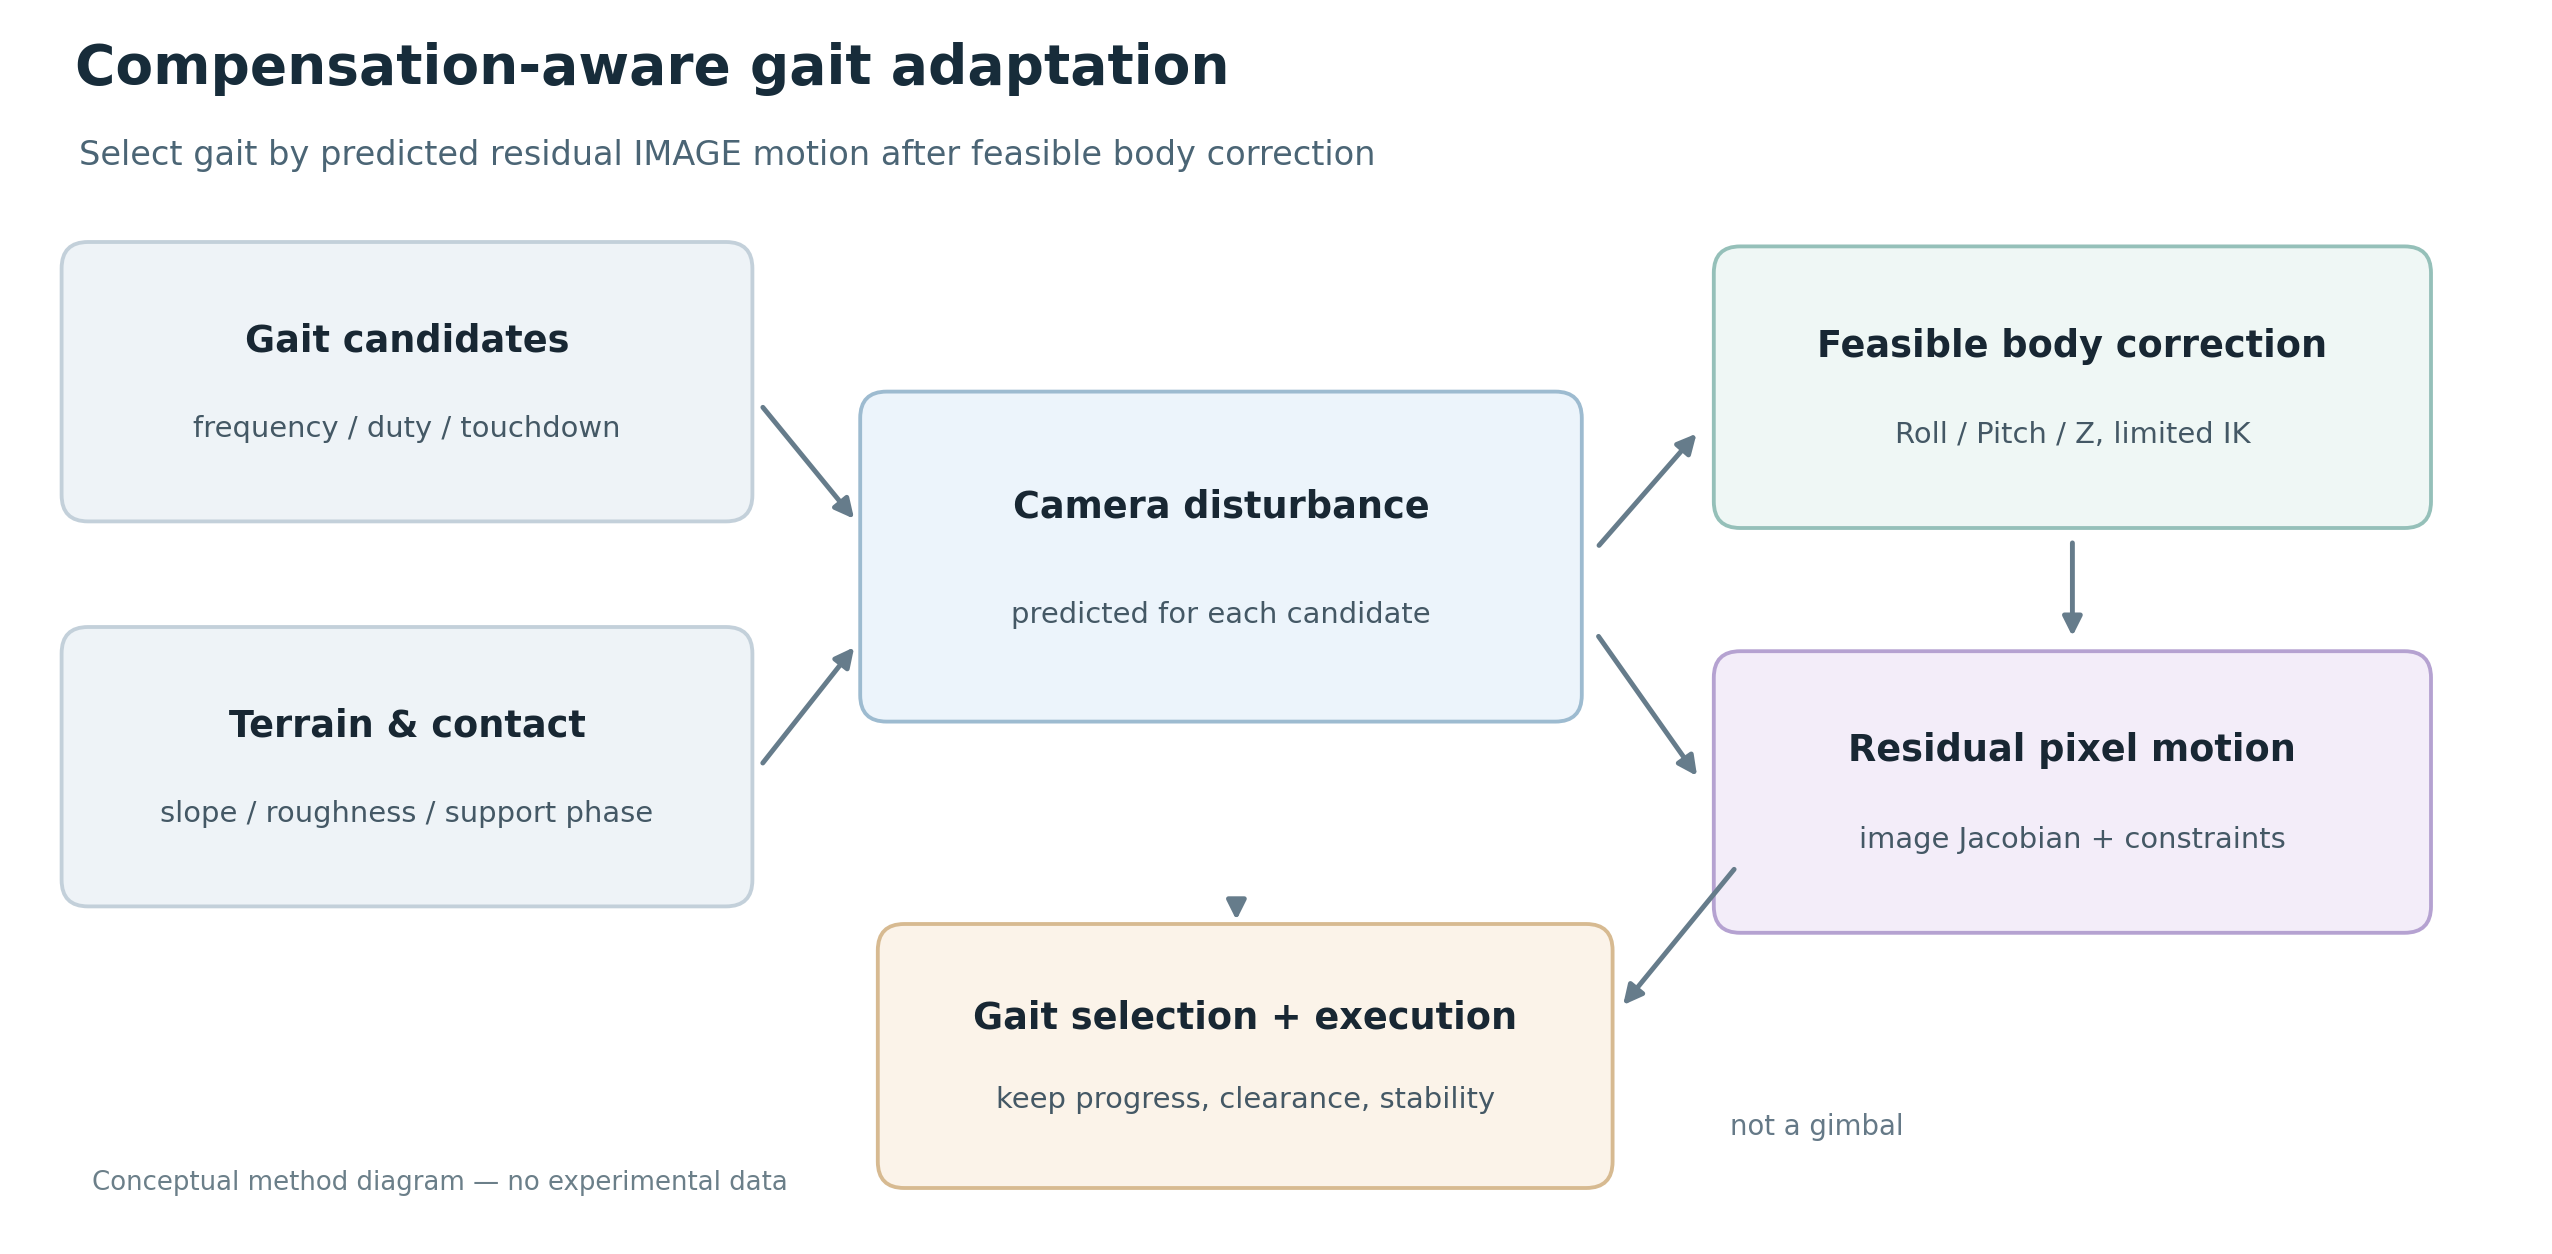
\includegraphics[width=\linewidth]{figures/Fig1_concept.png}
\caption{Research concept: a shared set of feasible gait candidates is evaluated using predicted gait-induced disturbance and the actual response of a fixed body stabilizer. The figure illustrates the proposed architecture and contains no experimental results.}\label{fig:concept}
\end{figure}

\subsection{Candidate generation and safe transitions}
We retain a phase-continuous alternating-tripod generator with gait parameters $\bm\theta=[f,\beta,\kappa]^\top$, where $f$ is cycle frequency, $\beta$ is the stance duty ratio, and $\kappa$ controls touchdown smoothness. The stride length is determined in conjunction with frequency and requested velocity rather than varied independently without regard to achieved speed. Swing height is set from required terrain clearance. A small neighborhood of candidate parameters is enumerated only at phase-safe transitions. The current gait and a verified fallback are always included.

The common locomotion layer checks joint position and velocity limits, stance-foot reachability, swing-foot clearance, and a support/contact safety condition for each candidate. Feasible correction is not inferred merely from available joint angle range. In particular, the nominally permissible body adjustment may still be impossible under foot-ground contact or actuator-response constraints. The online selector is never permitted to override the underlying safety controller.

\subsection{Gait-conditioned raw and closed-loop response prediction}
Let $\bm o_t$ collect only information available before choosing a gait: current joint and inertial states, gait phase, the preceding gait and time since the last change, available local terrain estimates, and predicted support/kinematic margins computed from the candidate trajectory. For the same candidate $\bm\theta$, we distinguish uncompensated disturbance $\bm d^{0,\bm\theta}$ from the residual $\bm r^{\pi,\bm\theta}$ when a \emph{fixed, physically executed} body-pose controller $\pi_c$ is enabled. Both are defined relative to the intended smooth camera motion from Section~\ref{sec:problem}; deliberate translation and navigation yaw are not treated as gait jitter.

A general candidate-conditioned formulation is
\begin{align}
\widehat{\bm d}^{0,\bm\theta}_{t:t+H}&=F_\psi(\bm o_t,\bm\theta,\widehat{\mathcal T}_t),\label{eq:predictor}\\
\widehat{\bm r}^{\pi,\bm\theta}_{t:t+H}&=G_\eta(\bm o_t,\bm\theta,\widehat{\bm d}^{0,\bm\theta}_{t:t+H};\pi_c).\label{eq:empiricalresponse}
\end{align}
Unlike an ideal inner minimization, $G_\eta$ must represent the \emph{achieved} response of $\pi_c$, including finite tracking bandwidth, support transitions and saturation. It need not assume that any kinematically reachable compensation command can be executed instantaneously.

The first executable surrogate predicts the short-window scalar image-motion costs $\widehat J^0(\bm o_t,\bm\theta)$ and $\widehat J^\pi(\bm o_t,\bm\theta)$ independently using small regularized regressors. These are trained on paired \emph{conditions} with the same gait parameterization, target speed, terrain realization and initial-state distribution, with the body stabilizer disabled/enabled, respectively. Such paired rollouts are not asserted to have identical subsequent robot trajectories. The effective reduction
\begin{equation}\label{eq:authorityproxy}
\widehat{\Delta J}_{\pi}(\bm\theta)=\widehat J^0(\bm\theta)-\widehat J^\pi(\bm\theta)
\end{equation}
is a measurable, controller-conditioned \emph{response proxy}, not a geometric wrench polytope or a proof of dynamic feasibility. It is allowed to be negative if compensation worsens camera stability. A separate regressor estimates the attained forward speed for candidate screening. Higher-dimensional camera-twist and multi-frequency models will be used only if their validation establishes additional value over this explicit baseline.

Crucially, the training observations must span \emph{different candidate gait settings}. Replaying the currently observed IMU trace under every candidate does not produce a counterfactual gait predictor. The training/test split is grouped by independent terrain realizations and seeds, and paired controller-on/off trials must remain in the same split. No future simulator contact state, privileged terrain ground truth or test-rollout achieved speed may be used as an online predictor input.

\subsection{Measured and support-dependent body response}
The same Roll, Pitch and vertical-body stabilization controller $\pi_c$ operates under every comparison method. Let $\bm b=[\delta z,\delta\phi,\delta\vartheta]^\top$ be its limited pose correction. For stance foot $i$ with an approximately fixed world contact point $\bm p_i^W$, the required leg-frame target is
\begin{equation}\label{eq:stanceanchor}
\bm p_i^B(\bm b)=\bm R_{WB}(\bm b)^\top(\bm p_i^W-\bm t_{WB}(\bm b)).
\end{equation}
The inverse kinematics must respect
\begin{equation}\label{eq:limits}
\bm q_{\min}\le\mathrm{IK}(\bm p_i^B)\le\bm q_{\max},\qquad
|\Delta\bm q_i|\le\dot{\bm q}_{\max}\Delta t.
\end{equation}
These are necessary but not sufficient conditions. Contact retention, slip, support margin and actual actuator response must also be checked or measured. Rather than inventing a frequency cut-off, we propose identification of the response between limited safe body-pose references and measured body/camera motion, with support conditions recorded. The empirical response model captures the effects of the existing controller in the tested domain; generality beyond observed speeds, surfaces and support states is not assumed.

\subsection{Residual image motion and supervisory decision}
Let $J^\pi(\bm\theta)$ measure unwanted image-plane motion \emph{after} the actual body compensator, obtained by projecting camera twist relative to the nominal motion through the image interaction matrix in Eq.~\eqref{eq:interaction} and integrating over camera frames. The projected per-frame RMS displacement is a reproducible kinematic proxy, not an actual photometric blur measurement. Independently recorded RGB trajectories provide the final visual metric by tracking static scene features and subtracting intentional navigation flow. Camera exposure, temporal synchronization and rolling-shutter effects must be controlled or reported.

The gait selection objective is
\begin{equation}\label{eq:outer_goal_new}
\begin{aligned}
\bm\theta_t^*=\arg\min_{\bm\theta\in\Theta_{\rm safe}}\quad
&\widehat J^\pi(\bm o_t,\bm\theta)+\lambda_s\|\bm\theta-\bm\theta_{t-1}\|_{\bm W}^2,\\
\mathrm{s.t.}\quad&\widehat v(\bm o_t,\bm\theta)\ge v_{\min}.
\end{aligned}
\end{equation}
Every candidate must first pass the same kinematic, contact and transition screens. The speed predictor is only a screening aid; measured achieved speed and traversal success remain decisive evidence. Parameter switching is restricted to safe phase boundaries and uses hysteresis to prevent chattering. If no candidate is admissible, the host controller retains its verified gait or stops safely.

\noindent\textbf{Algorithm 1:}\enspace At a gait update, (1) create a common, physically screened gait menu; (2) use the current state and locally available terrain estimates to predict short-window $\widehat J^0$, $\widehat J^\pi$ and achieved speed for each candidate; (3) reject candidates failing speed and support constraints; (4) select the feasible minimum of Eq.~\eqref{eq:outer_goal_new}; (5) enact parameter changes at a safe support transition while the unchanged fast body controller continues to run. The comparison selector differs \emph{only} by ranking candidates with $\widehat J^0$ instead of $\widehat J^\pi$.

\subsection{Identification, computational cost and scope}
We evaluate both predictors on held-out terrain realizations with absolute image-motion error, predicted ordering accuracy and top-one candidate regret; reporting averaged regression fit alone is insufficient. A dedicated mechanism study measures how frequently raw-motion and closed-loop-motion orderings differ across all candidate pairs, rather than showcasing a single favorable episode. An additional history-only residual-feedback selector determines whether counterfactual prediction improves adaptation beyond simple online tuning from previously executed gaits.

The current implementation uses a small standardized ridge model and finite menu search to keep computational overhead measurable. The number of evaluated candidates, mean and worst-case CPU time, rejected candidates and actual control-loop delay must be recorded on the target processor. This is a proposed method subject to evaluation, not a claimed real-time or performance result.

\section{Experimental Setup}\label{sec:experiments}
\subsection{Platform and terrain conditions}
The primary evidence will be obtained from the existing PCR-Net 18-DOF hexapod model and Isaac Gym/PhysX dynamics environment, with calibrated camera optical-frame extrinsics. Disturbance-response model development, identification, gait scheduling, ablations and held-out terrain evaluations will all use simulation data only. Robot dimensions, mass, actual control frequency, joint gains, contact parameters and camera calibration are \todoexp{verify exact values and commit identifiers from experiment configuration}. Four terrain families are specified: horizontal flat ground, slopes, procedurally uneven ground and discrete obstacle strips. Difficulty and terrain seeds must be defined before collecting final method comparisons.

A deliberately limited sim-to-real assessment will use the existing physical hexapod carrying an Intel RealSense D435i and an IMU. The model parameters and gait menu will be frozen before the physical evaluation; recorded physical video will not be used to train the response predictor. RGB and IMU timestamps will be synchronized and camera exposure settings fixed or logged. The RGB stream provides an independent measured image-motion metric rather than treating attitude alone as a measure of image quality.

\subsection{Baselines and equal-compute comparisons}
\begin{table}[ht]
\centering\small
\caption{Required control comparisons. All comparisons use the same robot, navigation commands, feasible gait menu where applicable, and camera calibration.}\label{tab:baselines}
\begin{tabular}{@{}p{0.12\linewidth}p{0.52\linewidth}p{0.27\linewidth}@{}}
\toprule
ID & Control strategy & What it tests \\
\midrule
B0 & Fixed tripod gait, no body compensation & Raw reference \\
B1 & Fixed tripod gait + IMU pose stabilization & Standard body compensation \\
B2 & Best train-terrain fixed gait + same body stabilizer & Adaptation necessity \\
B3 & Online gait selector minimizing raw body disturbance + same stabilizer & Raw-motion optimization \\
B4 & Online gait selector minimizing uncompensated image motion + same stabilizer & Image cost alone \\
B5 & Residual-image selector using gait-independent closed-loop response estimate & Candidate-specific response value \\
B6 & History-only tuning using measured residual image motion + same body stabilizer & Predictive vs. reactive adaptation \\
Ours & Candidate-specific measured-response prediction + residual-image gait selection & Full proposed mechanism \\
\bottomrule
\end{tabular}
\end{table}

The optimized fixed gait B2 is selected using \emph{training terrains only}, not the test terrains. B3--B6 and Ours receive comparable state information and candidate budgets. To avoid unbalanced computational advantage, we record the number of candidates and measured average/worst-case runtime of the selectors.

\subsection{Image quality, motion and feasibility metrics}
The primary metric is per-frame RMS unwanted image displacement $E_{\mathrm{jitter}}$, computed with projected static scene features relative to the commanded smooth camera motion. A genuinely recorded RGB metric independently tracks fixed scene features (or fiducial markers) and estimates the corresponding undesired image displacement, with moving-object features excluded. This is essential to rule out improvement caused only by inaccuracies in a modeled image metric.

Additional image outcomes include exposure-period projected path length (proxy, not physical blur), real-frame feature tracking inlier rate, loss rate for a stationary visual landmark and, where calibrated and feasible, actual image sharpness indicators. Motion outcomes include achieved travel speed, path progress, time to completion, terrain success, minimum stance stability margin, foot clearance, joint feasibility violations and contact slippage. The change in speed between methods is explicitly reported; methods with meaningfully different achieved speeds are not interpreted as equal locomotion alternatives.

\subsection{Paired trials and train/test separation}
All principal comparisons are performed in Isaac Gym; physical evaluation is not required for training or full multi-terrain benchmarking. Every simulation baseline is evaluated on common terrain seeds, navigation commands, and initial conditions. The unit of replication is an independent rollout or terrain seed, not an individual frame. Model selection and gait tuning use separate training seeds, and a held-out set of terrain instances is locked before final comparisons. A practical protocol is 4 terrain families $\times$ 10 held-out terrain seeds $\times$ 8 methods, subject to actual compute availability; the exact final sample count will be reported without inflating it using correlated video frames.

For each paired condition, we will report median and interquartile range or mean and dispersion as appropriate, together with paired confidence intervals based on independent run units. Individual failures and feasibility violations will be included, not deleted as inconvenient outliers. The speed-matched relative jitter reduction versus the strongest comparator is
\begin{equation}
\Delta_{\mathrm{jit}}=100\%\left(1-\frac{E_{\mathrm{jitter}}^{\mathrm{Ours}}}{E_{\mathrm{jitter}}^{\mathrm{comparator}}}\right).
\end{equation}
No target improvement percentage is claimed as an observed result.

\subsection{Ablations and disturbance-model fidelity}
Four focused ablations test the new mechanism: (A1) candidate ranking uses raw disturbance instead of residual; (A2) all candidates share a fixed correction budget; (A3) gait-conditional disturbance prediction is replaced with a candidate-independent prediction; and (A4) actuator response limits are omitted. A1 and A2 are especially important because they isolate the two ingredients of compensation-aware gait ranking.

Prediction accuracy will be measured on held-out terrain using normalized camera-twist errors, projected residual pixel-motion errors and \emph{candidate ranking accuracy}. Only predicting average raw motion is inadequate if the optimizer cannot distinguish the better candidate. Across eligible held-out candidate pairs, we report the prevalence of raw-versus-compensated ranking reversals and the improvement from compensation-conditioned selection, rather than only showcasing one favorable example. Controller-on and controller-off trials are paired by scenario and gait, but need not have identical subsequent trajectories. In addition, simulations will vary motor response and latency, foot--ground friction and contact parameters within calibrated or explicitly documented uncertainty ranges. Ground-truth future contact forces are used only for offline diagnostics, never as online gait-selector features.

\subsection{Physical camera assessment}
The reduced physical-robot study will compare B2 (optimized fixed gait), B3 (raw-disturbance gait selection), and Ours on level floor with a mild disturbance and one representative safe uneven surface, with repeated traversals under comparable measured speeds and the same exposure settings. The initial plan is three methods, two environments and three repetitions (18 recorded sequences); the final replication count will follow observed variability and will be stated explicitly. The response model is trained exclusively on simulation data and will not be re-fitted using these physical trials. At minimum, it should provide synchronized IMU and RGB trajectories, estimated static-scene jitter, achieved speed and task completion records. Distortions arising from rolling-shutter timing must be acknowledged; a kinematic exposure-path proxy must not be presented as actual measured blur without additional image evidence.

\section{Results}\label{sec:results}
\noindent\todoexp{No hexapod dynamics runs or real-camera experiments have yet been generated for this manuscript. Do not use illustrative numerical tests as paper results.}
\subsection{Comparison across terrain and locomotion conditions}
Report per-terrain and aggregate undesired image displacement, exposure-motion proxy, achieved speed and traversal success for B0--B6 and Ours. Use paired terrain seeds. Figure~\ref{fig:resultmap} is a \emph{figure slot}, not an observed result.
\begin{figure}[ht]\centering
\fbox{\parbox[c][36mm][c]{0.88\linewidth}{\centering \textbf{Figure 2 -- DATA REQUIRED}\\ Per-terrain jitter and achieved speed, baseline versus proposed, paired seeds.}}
\caption{Required per-terrain performance comparison; plot only after real rollout metrics are available.}\label{fig:resultmap}
\end{figure}
\subsection{Compensation-dependent gait ranking}
Show at least one case in which the best raw-disturbance gait differs from the best residual-image-disturbance gait. Report the predicted and measured ranking, the support geometry and available joint correction margins. This panel is central to distinguishing the method from loss-function replacement.
\begin{figure}[ht]\centering
\fbox{\parbox[c][32mm][c]{0.88\linewidth}{\centering \textbf{Figure 3 -- DATA REQUIRED}\\ Same candidate set: raw camera motion, attainable body correction, residual pixel motion.}}
\caption{Required mechanism-level evidence; compare prediction to independently recorded motion.}\label{fig:ranking}
\end{figure}
\subsection{Ablation, prediction, computation and real video}
Provide a train/test-separated predictor accuracy table; component ablations (A1--A4); controller timing distribution including worst-case latency; and synchronized image/IMU comparisons from the physical camera. Failure cases and loss of perception tracking should be visible rather than excluded.
\begin{table}[ht]\centering\small
\caption{Results reporting template. Numeric cells remain deliberately empty pending real measurements.}
\begin{tabular}{@{}lllll@{}}\toprule Method & Jitter (px/frame) & Speed (m/s) & Success (\%) & Runtime (ms)\\\midrule
B1 & TBD & TBD & TBD & TBD\\
B2 & TBD & TBD & TBD & TBD\\
B3 & TBD & TBD & TBD & TBD\\
B4 & TBD & TBD & TBD & TBD\\
B5 & TBD & TBD & TBD & TBD\\
Ours & TBD & TBD & TBD & TBD\\\bottomrule
\end{tabular}\label{tab:resultplaceholder}\end{table}

\section{Discussion and Limitations}
\subsection{When compensation-aware ranking is useful}
The mechanism is expected to be most relevant when compensation workspace or response bandwidth differs across gait candidates. In an unconstrained regime with a near-perfect stabilizer, the extra gait selection criterion may produce little benefit. That regime is a legitimate limiting case and should be included in analysis rather than hidden.

The model can also fail when predicted disturbances are dominated by uncertain contact events or when the optimal gait lies outside the small candidate set. A physically reliable response must explicitly address low-bandwidth position servos, contact uncertainty and the limited directions of body correction. Merely allowing a six-dimensional virtual camera correction would overstate what the legged platform can accomplish.

\subsection{Measurement limitations and real-world interpretation}
Camera twist prediction can be related to image displacement only through a stated camera model and visible depth distribution. Inter-frame jitter, exposure-time path length, motion blur, rolling-shutter shear and perception accuracy are not interchangeable metrics. A feature-depth weighting that improves short-range targets may not minimize background image motion; this tradeoff should be discussed for the eventual task. The real-camera comparison is necessary for any explicit claim about recorded video stabilization.

\subsection{Scope of claimed contribution}
The work cannot claim to be the first hexapod controller with gaze feedback, the first gait smoother, the first CPG--MPC hierarchy, or the first visual objective in robot control. Any eventual novelty claim must be supported by measured improvement over residual-image-cost scheduling with a candidate-independent compensation budget, not solely by superiority to a naive fixed tripod gait.

\section{Conclusions}
A conclusion reporting performance will be written once comparative dynamics and physical-camera measurements have been obtained. The intended scientific question concerns the value of candidate-specific \emph{remaining} image motion under feasible body compensation, not the general possibility of visual feedback or gait adaptation.
\section*{Author Contributions}
\todoexp{confirm actual authors and CRediT roles.}
\section*{Funding}
\todoexp{provide verified grant names and identifiers; do not invent.}
\section*{Institutional Review Board and Informed Consent Statements}
Not applicable to robot-only experiments unless the final study includes identifiable human participants.
\section*{Data Availability Statement}
\todoexp{decide reproducible repository, datasets and camera logs with all coauthors.}
\section*{Conflicts of Interest}
\todoexp{confirm with all authors.}
\begin{thebibliography}{20}
\bibitem{shaw2019} Shaw, S.; Sartoretti, G.; Olkin, J.; Paivine, W.; Choset, H. Workspace CPG with Body Pose Control for Stable, Directed Vision during Omnidirectional Locomotion. \emph{Proc. IEEE Int. Conf. Robot. Autom.} \textbf{2019}, 6316--6322. \url{https://doi.org/10.1109/ICRA.2019.8794313}.
\bibitem{saggar2007} Saggar, M.; D'Silva, T.; Kohl, N.; Stone, P. Autonomous Learning of Stable Quadruped Locomotion. In \emph{RoboCup 2006: Robot Soccer World Cup X}; Springer, \textbf{2007}, 98--109. \url{https://doi.org/10.1007/978-3-540-74024-7_9}.
\bibitem{yin2024} Yin, Y.; Gao, F.; Sun, Q.; Zhao, Y.; Xiao, Y. Smart Gait: A Gait Optimization Framework for Hexapod Robots. \emph{Chin. J. Mech. Eng.} \textbf{2024}, \emph{37}, 15. \url{https://doi.org/10.1186/s10033-024-01000-0}.
\bibitem{burkus2022} Burkus, E.; Odry, A.; Awrejcewicz, J.; Kecskes, I.; Odry, P. Mechanical Design and a Novel Structural Optimization Approach for Hexapod Walking Robots. \emph{Machines} \textbf{2022}, \emph{10}, 466. \url{https://doi.org/10.3390/machines10060466}.
\bibitem{yu2025} Collaborative Optimization Control of Gravity Center and Pose of Hexapod Robot in Complex Terrains. \emph{Machines} \textbf{2025}, \emph{13}, 871. \url{https://doi.org/10.3390/machines13090871}.
\bibitem{liu2026} Liu, R.; Zhu, J.; Su, M.; Gu, X.; Fang, S.; Zheng, D.; Yang, H. Trajectory Tracking of Underwater Hexapod Robot Based on Model Predictive Control. \emph{Machines} \textbf{2026}, \emph{14}, 171. \url{https://doi.org/10.3390/machines14020171}.
\bibitem{gao2022} Gao, Q.; Xue, J.; Yan, H. Synergistic Motion Stability of a Scorpion-like Composite Robot. \emph{Machines} \textbf{2022}, \emph{10}, 834. \url{https://doi.org/10.3390/machines10100834}.
\bibitem{robic2024} Robic, M.; Fraisse, R.; Marchand, E.; Chaumette, F. QP-Based Visual Servoing Under Motion Blur-Free Constraint. \emph{IEEE Robot. Autom. Lett.} \textbf{2024}, \emph{9}, 8738--8745. \url{https://doi.org/10.1109/LRA.2024.3451394}.
\end{thebibliography}
\end{document}
